% Options for packages loaded elsewhere
\PassOptionsToPackage{unicode}{hyperref}
\PassOptionsToPackage{hyphens}{url}
%
\documentclass[
  man]{apa6}
\usepackage{amsmath,amssymb}
\usepackage{lmodern}
\usepackage{iftex}
\ifPDFTeX
  \usepackage[T1]{fontenc}
  \usepackage[utf8]{inputenc}
  \usepackage{textcomp} % provide euro and other symbols
\else % if luatex or xetex
  \usepackage{unicode-math}
  \defaultfontfeatures{Scale=MatchLowercase}
  \defaultfontfeatures[\rmfamily]{Ligatures=TeX,Scale=1}
\fi
% Use upquote if available, for straight quotes in verbatim environments
\IfFileExists{upquote.sty}{\usepackage{upquote}}{}
\IfFileExists{microtype.sty}{% use microtype if available
  \usepackage[]{microtype}
  \UseMicrotypeSet[protrusion]{basicmath} % disable protrusion for tt fonts
}{}
\makeatletter
\@ifundefined{KOMAClassName}{% if non-KOMA class
  \IfFileExists{parskip.sty}{%
    \usepackage{parskip}
  }{% else
    \setlength{\parindent}{0pt}
    \setlength{\parskip}{6pt plus 2pt minus 1pt}}
}{% if KOMA class
  \KOMAoptions{parskip=half}}
\makeatother
\usepackage{xcolor}
\IfFileExists{xurl.sty}{\usepackage{xurl}}{} % add URL line breaks if available
\IfFileExists{bookmark.sty}{\usepackage{bookmark}}{\usepackage{hyperref}}
\hypersetup{
  pdftitle={Contextual cuing in the presence of an overt instruction},
  pdfauthor={Tom Beesley1 \& David Luque2},
  pdflang={en-EN},
  pdfkeywords={keywords},
  hidelinks,
  pdfcreator={LaTeX via pandoc}}
\urlstyle{same} % disable monospaced font for URLs
\usepackage{graphicx}
\makeatletter
\def\maxwidth{\ifdim\Gin@nat@width>\linewidth\linewidth\else\Gin@nat@width\fi}
\def\maxheight{\ifdim\Gin@nat@height>\textheight\textheight\else\Gin@nat@height\fi}
\makeatother
% Scale images if necessary, so that they will not overflow the page
% margins by default, and it is still possible to overwrite the defaults
% using explicit options in \includegraphics[width, height, ...]{}
\setkeys{Gin}{width=\maxwidth,height=\maxheight,keepaspectratio}
% Set default figure placement to htbp
\makeatletter
\def\fps@figure{htbp}
\makeatother
\setlength{\emergencystretch}{3em} % prevent overfull lines
\providecommand{\tightlist}{%
  \setlength{\itemsep}{0pt}\setlength{\parskip}{0pt}}
\setcounter{secnumdepth}{-\maxdimen} % remove section numbering
% Make \paragraph and \subparagraph free-standing
\ifx\paragraph\undefined\else
  \let\oldparagraph\paragraph
  \renewcommand{\paragraph}[1]{\oldparagraph{#1}\mbox{}}
\fi
\ifx\subparagraph\undefined\else
  \let\oldsubparagraph\subparagraph
  \renewcommand{\subparagraph}[1]{\oldsubparagraph{#1}\mbox{}}
\fi
\newlength{\cslhangindent}
\setlength{\cslhangindent}{1.5em}
\newlength{\csllabelwidth}
\setlength{\csllabelwidth}{3em}
\newlength{\cslentryspacingunit} % times entry-spacing
\setlength{\cslentryspacingunit}{\parskip}
\newenvironment{CSLReferences}[2] % #1 hanging-ident, #2 entry spacing
 {% don't indent paragraphs
  \setlength{\parindent}{0pt}
  % turn on hanging indent if param 1 is 1
  \ifodd #1
  \let\oldpar\par
  \def\par{\hangindent=\cslhangindent\oldpar}
  \fi
  % set entry spacing
  \setlength{\parskip}{#2\cslentryspacingunit}
 }%
 {}
\usepackage{calc}
\newcommand{\CSLBlock}[1]{#1\hfill\break}
\newcommand{\CSLLeftMargin}[1]{\parbox[t]{\csllabelwidth}{#1}}
\newcommand{\CSLRightInline}[1]{\parbox[t]{\linewidth - \csllabelwidth}{#1}\break}
\newcommand{\CSLIndent}[1]{\hspace{\cslhangindent}#1}
\ifLuaTeX
\usepackage[bidi=basic]{babel}
\else
\usepackage[bidi=default]{babel}
\fi
\babelprovide[main,import]{english}
% get rid of language-specific shorthands (see #6817):
\let\LanguageShortHands\languageshorthands
\def\languageshorthands#1{}
% Manuscript styling
\usepackage{upgreek}
\captionsetup{font=singlespacing,justification=justified}

% Table formatting
\usepackage{longtable}
\usepackage{lscape}
% \usepackage[counterclockwise]{rotating}   % Landscape page setup for large tables
\usepackage{multirow}		% Table styling
\usepackage{tabularx}		% Control Column width
\usepackage[flushleft]{threeparttable}	% Allows for three part tables with a specified notes section
\usepackage{threeparttablex}            % Lets threeparttable work with longtable

% Create new environments so endfloat can handle them
% \newenvironment{ltable}
%   {\begin{landscape}\centering\begin{threeparttable}}
%   {\end{threeparttable}\end{landscape}}
\newenvironment{lltable}{\begin{landscape}\centering\begin{ThreePartTable}}{\end{ThreePartTable}\end{landscape}}

% Enables adjusting longtable caption width to table width
% Solution found at http://golatex.de/longtable-mit-caption-so-breit-wie-die-tabelle-t15767.html
\makeatletter
\newcommand\LastLTentrywidth{1em}
\newlength\longtablewidth
\setlength{\longtablewidth}{1in}
\newcommand{\getlongtablewidth}{\begingroup \ifcsname LT@\roman{LT@tables}\endcsname \global\longtablewidth=0pt \renewcommand{\LT@entry}[2]{\global\advance\longtablewidth by ##2\relax\gdef\LastLTentrywidth{##2}}\@nameuse{LT@\roman{LT@tables}} \fi \endgroup}

% \setlength{\parindent}{0.5in}
% \setlength{\parskip}{0pt plus 0pt minus 0pt}

% Overwrite redefinition of paragraph and subparagraph by the default LaTeX template
% See https://github.com/crsh/papaja/issues/292
\makeatletter
\renewcommand{\paragraph}{\@startsection{paragraph}{4}{\parindent}%
  {0\baselineskip \@plus 0.2ex \@minus 0.2ex}%
  {-1em}%
  {\normalfont\normalsize\bfseries\itshape\typesectitle}}

\renewcommand{\subparagraph}[1]{\@startsection{subparagraph}{5}{1em}%
  {0\baselineskip \@plus 0.2ex \@minus 0.2ex}%
  {-\z@\relax}%
  {\normalfont\normalsize\itshape\hspace{\parindent}{#1}\textit{\addperi}}{\relax}}
\makeatother

% \usepackage{etoolbox}
\makeatletter
\patchcmd{\HyOrg@maketitle}
  {\section{\normalfont\normalsize\abstractname}}
  {\section*{\normalfont\normalsize\abstractname}}
  {}{\typeout{Failed to patch abstract.}}
\patchcmd{\HyOrg@maketitle}
  {\section{\protect\normalfont{\@title}}}
  {\section*{\protect\normalfont{\@title}}}
  {}{\typeout{Failed to patch title.}}
\makeatother

\usepackage{xpatch}
\makeatletter
\xapptocmd\appendix
  {\xapptocmd\section
    {\addcontentsline{toc}{section}{\appendixname\ifoneappendix\else~\theappendix\fi\\: #1}}
    {}{\InnerPatchFailed}%
  }
{}{\PatchFailed}
\keywords{keywords\newline\indent Word count: X}
\DeclareDelayedFloatFlavor{ThreePartTable}{table}
\DeclareDelayedFloatFlavor{lltable}{table}
\DeclareDelayedFloatFlavor*{longtable}{table}
\makeatletter
\renewcommand{\efloat@iwrite}[1]{\immediate\expandafter\protected@write\csname efloat@post#1\endcsname{}}
\makeatother
\usepackage{lineno}

\linenumbers
\usepackage{csquotes}
\raggedbottom
\usepackage[font={small,it}, labelfont={bf}]{caption}
\ifLuaTeX
  \usepackage{selnolig}  % disable illegal ligatures
\fi

\title{Contextual cuing in the presence of an overt instruction}
\author{Tom Beesley\textsuperscript{1} \& David Luque\textsuperscript{2}}
\date{}


\shorttitle{Contextual cuing and instruction}

\authornote{

Correspondence concerning this article should be addressed to Tom Beesley, Department of Psychology, Lancaster University, UK, LA1 4YD. E-mail: \href{mailto:t.beesley@lancaster.ac.uk}{\nolinkurl{t.beesley@lancaster.ac.uk}}

}

\affiliation{\vspace{0.5cm}\textsuperscript{1} Lancaster University, UK\\\textsuperscript{2} Universidad Autónoma de Madrid, Spain}

\abstract{%
abstract here

Public significance statement:
}



\begin{document}
\maketitle

Main text here (Beesley et al., 2015)

\begin{verbatim}
## # A tibble: 3 x 2
##   exp   num_Ps
##   <fct>  <int>
## 1 CCC01     31
## 2 CCC02     34
## 3 CCC03     43
\end{verbatim}

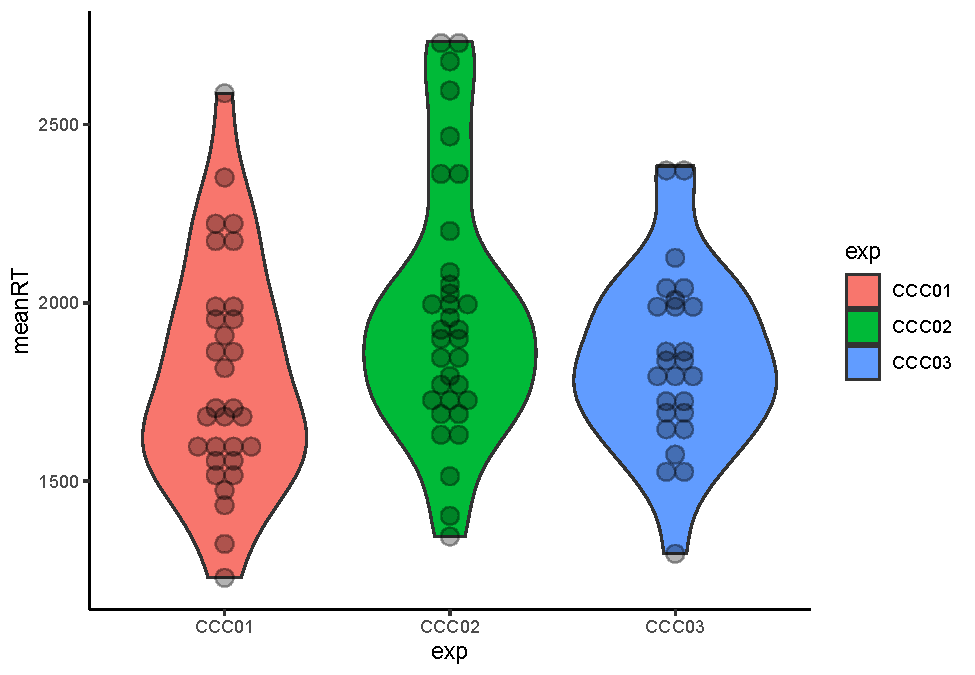
\includegraphics{CCC_ms1_files/figure-latex/unnamed-chunk-1-1.pdf} 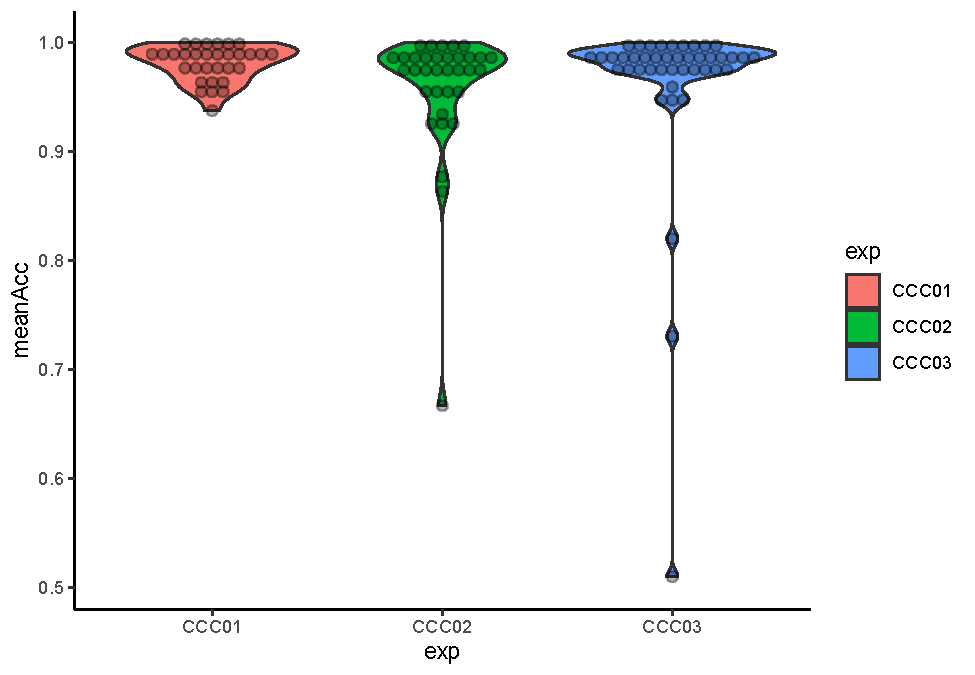
\includegraphics{CCC_ms1_files/figure-latex/unnamed-chunk-1-2.pdf}

\hypertarget{experiment-1}{%
\section{Experiment 1}\label{experiment-1}}

Experiment 1 sought to examine whether the learnt attentional behaviour developed contextual cuing was expressed when participants were directed with a top-down instruction to search in a particular region of the search space. Participants were first trained with a set of four repeating configurations

\hypertarget{method}{%
\subsection{Method}\label{method}}

\hypertarget{participants}{%
\subsubsection{Participants}\label{participants}}

Thirty-one undergraduate students from Lancaster University were recruited (mean age = 20.13, SD = 1.09; 17 identified as male and 14 as female) via the Psychology Research Participation System in the Department of Psychology at Lancaster University, in return for the opportunity to use the recruitment system for their own research in future years.

\hypertarget{materials}{%
\subsubsection{Materials}\label{materials}}

Participants were tested individually in a quiet room with a Dell laptop with a 15.6'' screen, a screen resolution of 1920 x 1080, and a full size external keyboard for participants to use to respond to the task. Participants sat approximately 50 cm from the screen. Stimulus presentation was controlled by MATLAB using the Psychophysics Toolbox extensions (Brainard, 1997; Kleiner, Brainard \& Pelli, 2007; Pelli, 1997). Responses to the target stimulus were made by pressing the `c' or `n' key on a standard keyboard. All experimental materials are available at the github repository for this study.

Distractor stimuli were an `L' shape (rotated 0°, 90°, 180°, or 270°) while the target stimulus was a `T' shape (rotated at either 90° or 270°). Stimuli were arranged in a square grid of 144 evenly spaced cells (12 x 12) which was positioned centrally on the screen and was XXX mm (XX°) square. The grid itself was invisible to participants. The fixation cross (displayed centrally before each trial) was XX mm (X.X°) square. The stimuli were XX mm (X.X°) square. The background of the screen was grey (RGB: .6, .6, .6) and the stimuli were presented in black. There was a small offset in the vertical line of the `L' distractors, which increased the similarity between the `L' distractor and the target `T', making the search task more difficult (Duncan \& Humphreys, 1989).

\hypertarget{design}{%
\subsubsection{Design}\label{design}}

\hypertarget{procedure}{%
\subsubsection{Procedure}\label{procedure}}

\hypertarget{results}{%
\subsection{Results}\label{results}}

Our criterion for removing outlier data, at both the participant level and the trial level, was 2.5 standard deviations above or below the mean of the sample. On average, trials ended with a timeout on 1.97\% of trials (SD = 2.53). Two participants had an usually high proportion of timeouts and were removed from the analysis. The mean accuracy of participants (not including timeout trials) was 98.10\% (SD = 1.65\%). One participants that had an unusually low proportion of accurate trials and were also removed. The only participant deemed to be an outlier in terms of mean response time (hereafter RT) was also excluded on the basis of the timeout criterion, noted above.

For the remaining twenty-eight participants we removed trials with a timeout and inaccurate trials, before removing outliers from the RT data. On average, the proportion of outliers removed was 3.03\% (SD = 0.79\%). zero participants had an unusual proportion of trials removed as outlier RTs.

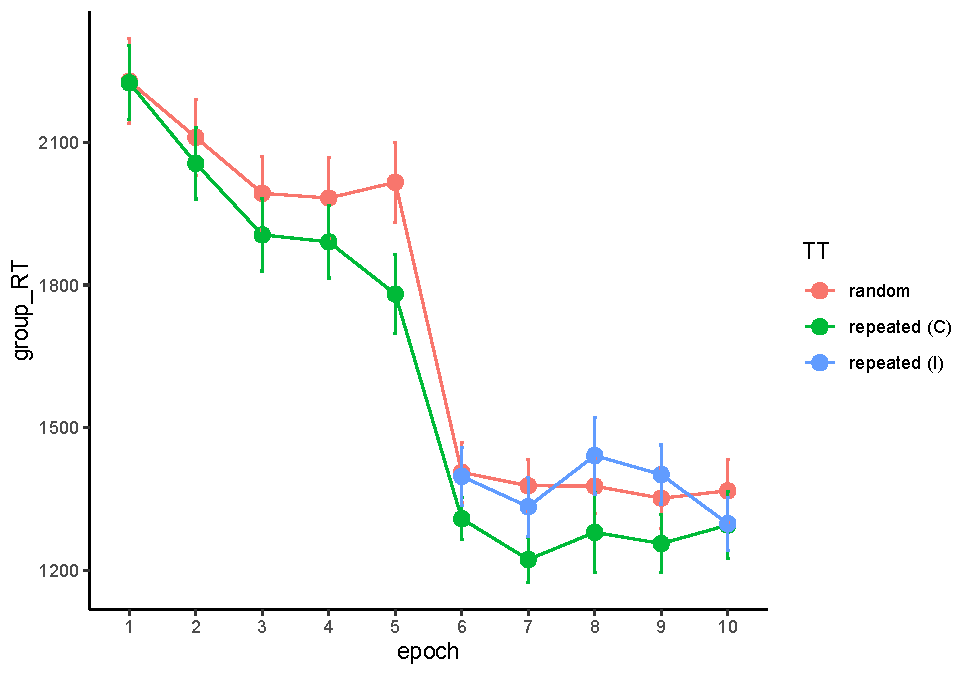
\includegraphics{CCC_ms1_files/figure-latex/unnamed-chunk-5-1.pdf}

\begin{verbatim}
## Anova Table (Type 3 tests)
## 
## Response: meanRT
##     Effect          df      MSE         F  ges p.value
## 1       TT       1, 27 83590.71    7.48 * .013    .011
## 2    epoch 3.66, 98.95 65143.51 17.25 *** .078   <.001
## 3 TT:epoch 3.30, 89.04 41403.04    3.05 * .008    .029
## ---
## Signif. codes:  0 '***' 0.001 '**' 0.01 '*' 0.05 '+' 0.1 ' ' 1
## 
## Sphericity correction method: GG
\end{verbatim}

\begin{verbatim}
## Anova Table (Type 3 tests)
## 
## Response: meanRT
##     Effect           df       MSE       F  ges p.value
## 1       TT  1.95, 52.75  70324.29 7.17 ** .021    .002
## 2    epoch  2.18, 58.91 125085.52    0.88 .005    .430
## 3 TT:epoch 5.14, 138.75  48674.61    1.22 .007    .304
## ---
## Signif. codes:  0 '***' 0.001 '**' 0.01 '*' 0.05 '+' 0.1 ' ' 1
## 
## Sphericity correction method: GG
\end{verbatim}

\begin{verbatim}
## 
##  Welch Two Sample t-test
## 
## data:  meanRT by TT
## t = 2.6582, df = 277.56, p-value = 0.008311
## alternative hypothesis: true difference in means between group random and group repeated (C) is not equal to 0
## 95 percent confidence interval:
##   26.83853 180.04444
## sample estimates:
##       mean in group random mean in group repeated (C) 
##                   1376.039                   1272.598
\end{verbatim}

\begin{verbatim}
## 
##  Welch Two Sample t-test
## 
## data:  meanRT by TT
## t = 0.037309, df = 276.73, p-value = 0.9703
## alternative hypothesis: true difference in means between group random and group repeated (I) is not equal to 0
## 95 percent confidence interval:
##  -76.27970  79.22693
## sample estimates:
##       mean in group random mean in group repeated (I) 
##                   1376.039                   1374.566
\end{verbatim}

\begin{verbatim}
## 
##  Welch Two Sample t-test
## 
## data:  meanRT by TT
## t = -2.5333, df = 277.78, p-value = 0.01185
## alternative hypothesis: true difference in means between group repeated (C) and group repeated (I) is not equal to 0
## 95 percent confidence interval:
##  -181.20322  -22.73253
## sample estimates:
## mean in group repeated (C) mean in group repeated (I) 
##                   1272.598                   1374.566
\end{verbatim}

\hypertarget{experiment-2}{%
\section{Experiment 2}\label{experiment-2}}

Experiment 2 sought to examine \ldots{}

\hypertarget{method-1}{%
\subsection{Method}\label{method-1}}

\hypertarget{participants-1}{%
\subsubsection{Participants}\label{participants-1}}

Thirty-one undergraduate students from Lancaster University were recruited (mean age = 20.13, SD = 1.09; 17 identified as male and 14 as female) via the Psychology Research Participation System in the Department of Psychology at Lancaster University, in return for the opportunity to use the recruitment system for their own research in future years.

\hypertarget{materials-1}{%
\subsubsection{Materials}\label{materials-1}}

The materials and stimuli were identical to Experiment 1.

\hypertarget{design-1}{%
\subsubsection{Design}\label{design-1}}

\hypertarget{procedure-1}{%
\subsubsection{Procedure}\label{procedure-1}}

\hypertarget{results-1}{%
\subsection{Results}\label{results-1}}

Our criteria for removing outlier data were identical to Experiment 1. On average, trials ended with a timeout on 2.13\% of trials (SD = 1.83). Zero participants had an usually high proportion of timeouts. The mean accuracy of participants (not including timeout trials) was 95.85\% (SD = 6.10\%). One participants that had an unusually low proportion of accurate trials and were also removed. Zero participants were deemed to be an outlier in terms of mean RT.

For the remaining thirty-three participants we removed trials with a timeout and inaccurate trials, before removing outliers from the RT data. On average, the proportion of outliers removed was 2.81\% (SD = 1.04\%). one participants had an unusual proportion of trials removed as outlier RTs and were not included in the final analysis.

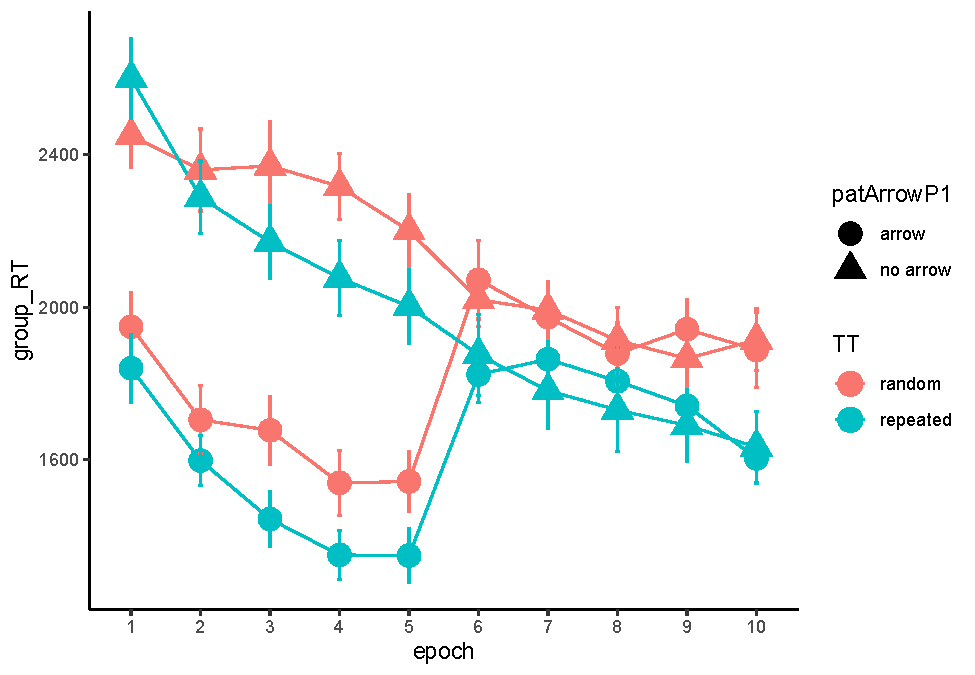
\includegraphics{CCC_ms1_files/figure-latex/unnamed-chunk-11-1.pdf}

\begin{verbatim}
## Anova Table (Type 3 tests)
## 
## Response: meanRT
##                Effect           df       MSE          F   ges p.value
## 1          patArrowP1        1, 32 442144.07 175.06 ***  .313   <.001
## 2                  TT        1, 32 151825.16  21.10 ***  .019   <.001
## 3               epoch 3.13, 100.03 200796.66  24.76 ***  .084   <.001
## 4       patArrowP1:TT        1, 32 164480.86       0.74 <.001    .395
## 5    patArrowP1:epoch 3.34, 107.03 147265.04       0.61  .002    .630
## 6            TT:epoch 3.48, 111.28  89997.46    4.53 **  .008    .003
## 7 patArrowP1:TT:epoch 3.39, 108.43  62430.81     2.24 +  .003    .080
## ---
## Signif. codes:  0 '***' 0.001 '**' 0.01 '*' 0.05 '+' 0.1 ' ' 1
## 
## Sphericity correction method: GG
\end{verbatim}

\begin{verbatim}
## Bayes factor analysis
## --------------
## [1] patArrowP1 + TT + patArrowP1:TT + subj : 0.188733 ±5.65%
## 
## Against denominator:
##   meanRT ~ patArrowP1 + TT + subj 
## ---
## Bayes factor type: BFlinearModel, JZS
\end{verbatim}

\begin{verbatim}
## Anova Table (Type 3 tests)
## 
## Response: meanRT
##                Effect           df       MSE         F   ges p.value
## 1          patArrowP1        1, 32 107851.75      0.48 <.001    .493
## 2                  TT        1, 32 117763.13 51.20 ***  .035   <.001
## 3               epoch 3.44, 109.95  79887.36 10.79 ***  .017   <.001
## 4       patArrowP1:TT        1, 32 284015.04      0.04 <.001    .850
## 5    patArrowP1:epoch 3.58, 114.51  94104.45      0.47 <.001    .737
## 6            TT:epoch 3.39, 108.54  89788.68      1.46  .003    .227
## 7 patArrowP1:TT:epoch 3.70, 118.33  97123.16      0.75  .002    .549
## ---
## Signif. codes:  0 '***' 0.001 '**' 0.01 '*' 0.05 '+' 0.1 ' ' 1
## 
## Sphericity correction method: GG
\end{verbatim}

\begin{verbatim}
## Bayes factor analysis
## --------------
## [1] patArrowP1 + TT + patArrowP1:TT + subj : 0.1283105 ±2.37%
## 
## Against denominator:
##   meanRT ~ patArrowP1 + TT + subj 
## ---
## Bayes factor type: BFlinearModel, JZS
\end{verbatim}

\hypertarget{experiment-3}{%
\section{Experiment 3}\label{experiment-3}}

Experiment 3 sought to examine \ldots{}

\hypertarget{method-2}{%
\subsection{Method}\label{method-2}}

\hypertarget{participants-2}{%
\subsubsection{Participants}\label{participants-2}}

Forty-three undergraduate students from Lancaster University were recruited (mean age = 18.65, SD = 2.81; 29 identified as male and 12 as female) via the Psychology Research Participation System in the Department of Psychology at Lancaster University, in return for the opportunity to use the recruitment system for their own research in future years.

\hypertarget{materials-2}{%
\subsubsection{Materials}\label{materials-2}}

The materials and stimuli were identical to Experiment 1.

\hypertarget{design-2}{%
\subsubsection{Design}\label{design-2}}

\hypertarget{procedure-2}{%
\subsubsection{Procedure}\label{procedure-2}}

\hypertarget{results-2}{%
\subsection{Results}\label{results-2}}

Our criteria for removing outlier data were identical to Experiment 1. On average, trials ended with a timeout on 3.33\% of trials (SD = 4.08). One participants had an usually high proportion of timeouts. The mean accuracy of participants (not including timeout trials) was 96.12\% (SD = 8.47\%). Two participants that had an unusually low proportion of accurate trials and were also removed. Zero participants were deemed to be an outlier in terms of mean RT.

For the remaining forty participants we removed trials with a timeout and inaccurate trials, before removing outliers from the RT data. On average, the proportion of outliers removed was 3.13\% (SD = 0.72\%). zero participants had an unusual proportion of trials removed as outlier RTs and were not included in the final analysis {[}EAF4S{]}.

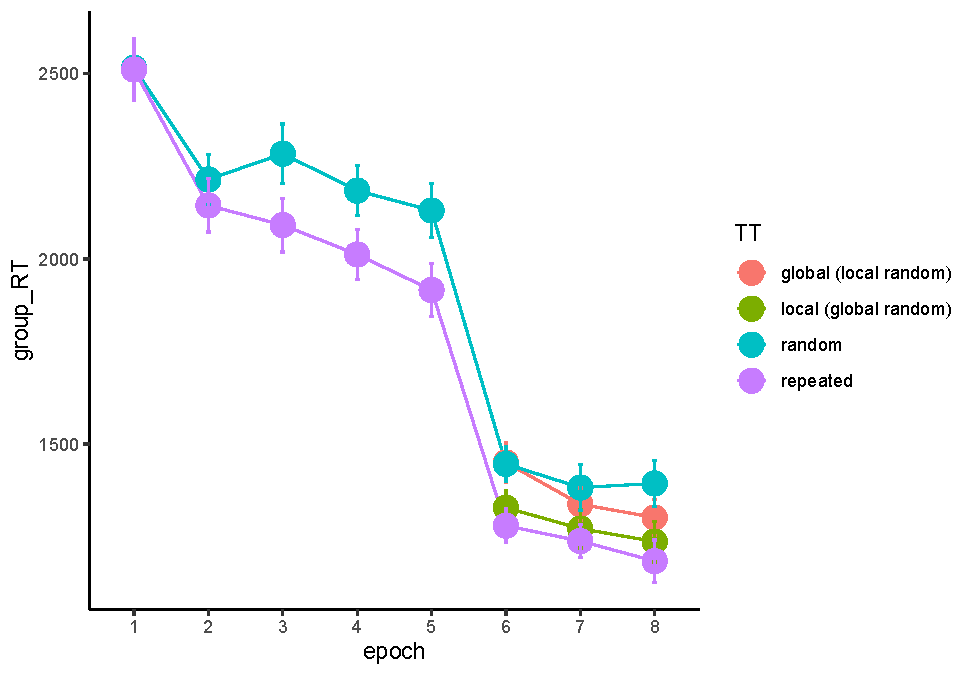
\includegraphics{CCC_ms1_files/figure-latex/unnamed-chunk-17-1.pdf}

\begin{verbatim}
## Anova Table (Type 3 tests)
## 
## Response: meanRT
##     Effect           df       MSE         F  ges p.value
## 1       TT        1, 39  84371.29 20.35 *** .021   <.001
## 2    epoch 3.41, 132.99 110399.09 29.89 *** .121   <.001
## 3 TT:epoch 3.69, 144.06  67824.76    2.57 * .008    .045
## ---
## Signif. codes:  0 '***' 0.001 '**' 0.01 '*' 0.05 '+' 0.1 ' ' 1
## 
## Sphericity correction method: GG
\end{verbatim}

\begin{verbatim}
## Anova Table (Type 3 tests)
## 
## Response: meanRT
##     Effect           df      MSE         F  ges p.value
## 1       TT 2.71, 105.61 31057.96 26.59 *** .043   <.001
## 2    epoch  1.78, 69.46 51362.09  8.72 *** .016   <.001
## 3 TT:epoch 4.44, 173.24 38443.76      0.77 .003    .558
## ---
## Signif. codes:  0 '***' 0.001 '**' 0.01 '*' 0.05 '+' 0.1 ' ' 1
## 
## Sphericity correction method: GG
\end{verbatim}

\begin{verbatim}
## Bayes factor analysis
## --------------
## [1] TT + subj : 51224793199 ±0.64%
## 
## Against denominator:
##   meanRT ~ subj 
## ---
## Bayes factor type: BFlinearModel, JZS
\end{verbatim}

\begin{verbatim}
## Bayes factor analysis
## --------------
## [1] TT + subj : 0.8197581 ±1.61%
## 
## Against denominator:
##   meanRT ~ subj 
## ---
## Bayes factor type: BFlinearModel, JZS
\end{verbatim}

\begin{verbatim}
## Bayes factor analysis
## --------------
## [1] TT + subj : 1043053 ±0.84%
## 
## Against denominator:
##   meanRT ~ subj 
## ---
## Bayes factor type: BFlinearModel, JZS
\end{verbatim}

\begin{verbatim}
## Bayes factor analysis
## --------------
## [1] TT + subj : 10691.83 ±1.05%
## 
## Against denominator:
##   meanRT ~ subj 
## ---
## Bayes factor type: BFlinearModel, JZS
\end{verbatim}

\begin{verbatim}
## Bayes factor analysis
## --------------
## [1] TT + subj : 0.7432093 ±0.96%
## 
## Against denominator:
##   meanRT ~ subj 
## ---
## Bayes factor type: BFlinearModel, JZS
\end{verbatim}

\begin{verbatim}
## Bayes factor analysis
## --------------
## [1] TT + subj : 38.05145 ±0.85%
## 
## Against denominator:
##   meanRT ~ subj 
## ---
## Bayes factor type: BFlinearModel, JZS
\end{verbatim}

\begin{verbatim}
## 
##  Paired t-test
## 
## data:  meanRT by TT
## t = 4.0807, df = 119, p-value = 8.159e-05
## alternative hypothesis: true difference in means is not equal to 0
## 95 percent confidence interval:
##   43.40317 125.22884
## sample estimates:
## mean of the differences 
##                84.31601
\end{verbatim}

\newpage

\hypertarget{references}{%
\section*{References}\label{references}}
\addcontentsline{toc}{section}{References}

\hypertarget{refs}{}
\begin{CSLReferences}{1}{0}
\leavevmode\vadjust pre{\hypertarget{ref-beesley2015b}{}}%
Beesley, T., Vadillo, M. A., Pearson, D., \& Shanks, D. R. (2015). Pre-exposure of repeated search configurations facilitates subsequent contextual cuing of visual search. \emph{Journal of Experimental Psychology: Learning, Memory, and Cognition}, \emph{41}(2), 348--362. \url{https://doi.org/10.1037/xlm0000033}

\end{CSLReferences}


\end{document}
